\section{Расчёт критических кумулянтов для модели прямоугольного Изинга}

Кумулянт Биндера для модели Изинга в критической точке расчитывается по формуле:
\begin{equation}
\label{eq:Cumulant}
U_{4} = 1 - \frac{\la m^{4} \ra}{3 * (m^{2})^{2}}
\end{equation}

где $\la m^{2} \ra$ - средний квадрат удельной намагниченности, $\la m^{4} \ra$ - средная удельная намагниченность в четвертой степени. 

Для сравнения значения кумулянтов модели прямоугольного Изинга с разными размерами, но одинаковым отношением сторон (так же Aspect Ratio или r), так, что число спинов составляет L * rL были проведены симуляции модели на основе алгоритма из проектной работы Сорокина Никиты \cite{Schro} и Камиллы Файзулиной \cite{SAW} - для этого были взяты длины 50, 100, 200 и 400 и отношения сторон 1/4, 1/2, 3/4 при $2 * 10^{6}$ итераций.

\begin{figure}[!h]
    \centering
    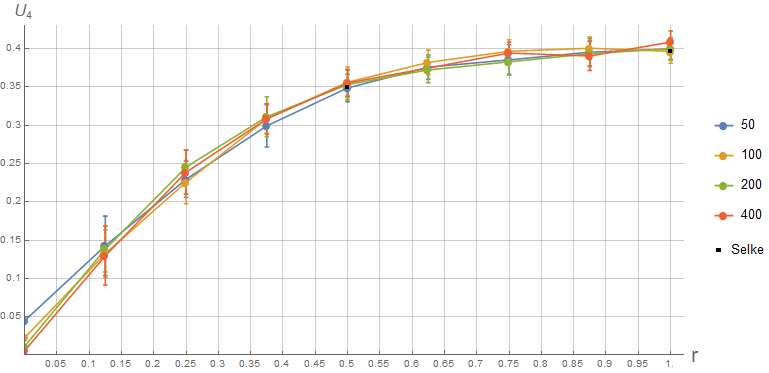
\includegraphics[width=100mm]{Sections/Images/CumulantOBC.png}
    \caption{График зависимости значения кумулянта Биндера в крит. точке от Aspect Ratio при открытых гран. условиях}
    \label{fig:CumulOBC}
\end{figure}

\begin{figure}[!h]
    \centering
    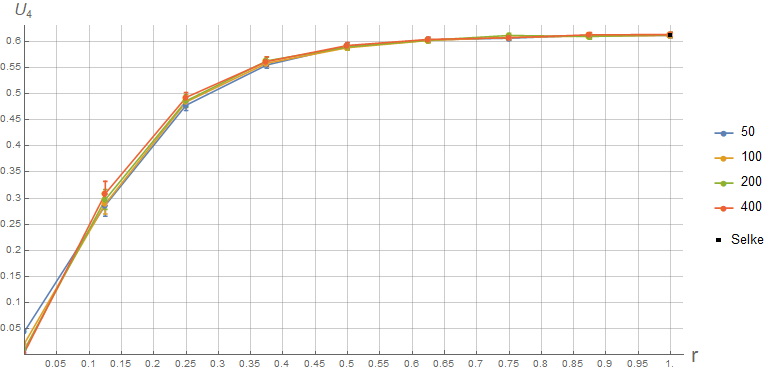
\includegraphics[width=100mm]{Sections/Images/CumulantPBC.png}
    \caption{График зависимости значения кумулянта Биндера в крит. точке от Aspect Ratio при периодических гран. условиях}
    \label{fig:CumulPBC}
\end{figure}

Крайние левые точки в отметке нуля являются расчётами для модели одномерного Изинга (где длина цепочки равна соответствующей стороне в двумерном изинге). Так, в случае открытых гран. условий (рис. \ref{fig:CumulOBC}) и периодических (рис. \ref{fig:CumulPBC}) значения кумулянта стремится к нулю с увеличением длины цепочки(см. Проект6.pdf\cite{Git}).
Черными точками отмечены значения критического кумулянта из работы Уолтера Сельке - 0.396 ± 0.002 для квадратной модели и 0.349 ± 0.002 для прямоугольной с отношением сторон r = 1/2 при открытых гран. условий. Для периодического случая квадратной модели критический кумулянт равен 0.61069\cite{Selke}.

Эти же значения отмечены в графиках \ref{fig:CumulOBCL} и \ref{fig:CumulPBCL} зависимости крит. кумулянта от обратной длины стороны как крайние левые (в нуле - так обозначен случай термодинамического предела).

\begin{figure}[!h]
    \centering
    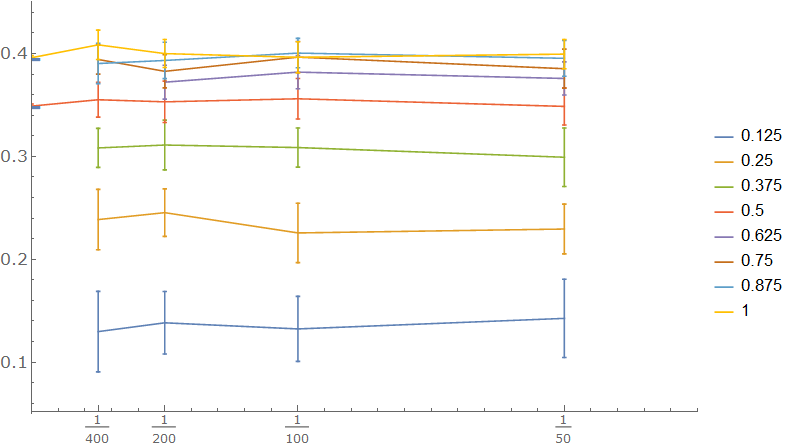
\includegraphics[width=100mm]{Sections/Images/CumulantOBCL.png}
    \caption{График зависимости значения кумулянта Биндера в крит. точке от обратной длины стороны при открытых гран. условиях}
    \label{fig:CumulOBCL}
\end{figure}

\begin{figure}[!h]
    \centering
    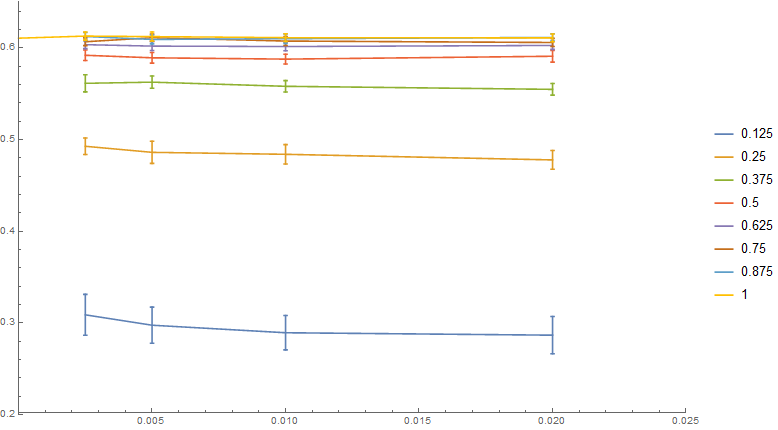
\includegraphics[width=100mm]{Sections/Images/CumulantPBCL.png}
    \caption{График зависимости значения кумулянта Биндера в крит. точке от обратной длины стороны при периодических гран. условиях}
    \label{fig:CumulPBCL}
\end{figure}

Учитывая погрешность в расчётах симуляций, зависимость от обратной длины прямоугольника 1/L не наблюдается.